\documentclass[aspectratio=169,10pt]{beamer}
\usetheme{default}
\usecolortheme{seagull}
\setbeamertemplate{navigation symbols}{}
\setbeamertemplate{footline}[frame number]
\setbeamerfont{frametitle}{series=\bfseries,size=\large}
\setbeamercolor{frametitle}{fg=black}
\usepackage{tikz,booktabs,amsmath,amssymb,array}
\usetikzlibrary{positioning,arrows.meta,fit,calc}

\definecolor{cblue}{HTML}{2A78D6}
\definecolor{cgreen}{HTML}{16825D}
\definecolor{corange}{HTML}{C87800}
\definecolor{cviolet}{HTML}{4A3AA7}
\definecolor{cred}{HTML}{C43B3B}
\definecolor{cgray}{HTML}{555555}
\newcommand{\good}[1]{\textcolor{cgreen}{\textbf{#1}}}
\newcommand{\warn}[1]{\textcolor{corange}{\textbf{#1}}}
\newcommand{\bad}[1]{\textcolor{cred}{\textbf{#1}}}
\newcommand{\sg}{\operatorname{sg}}

\title{Latent World Models for Language Reasoning}
\subtitle{Action-conditioned prediction, counterfactual planning, and hierarchical control}
\author{TextJEPA project}
\date{July 14, 2026}

\begin{document}
\frame{\titlepage}

\begin{frame}{Question and approach}
\begin{columns}[T,onlytextwidth]
\column{0.48\textwidth}
\textbf{Question.} Can a reconstruction-free world model plan a language
reasoning trace by predicting consequences in latent space?

\medskip
\textbf{State.} Prompt plus outcomes established so far.

\textbf{Action.} A sentence describing the next reasoning intent, without its
computed result.

\textbf{Transition.} Predict the latent state after that intent is executed.
\column{0.48\textwidth}
\textbf{Evaluation.} At every step, enumerate the same feasible actions for
all methods, score them, execute one, observe its rendered outcome, and
replan.

\medskip
The central methodological question is which training objectives are
actually necessary for accurate action selection.
\end{columns}
\end{frame}

\begin{frame}{Reasoning as a controlled trajectory}
\small
\begin{center}
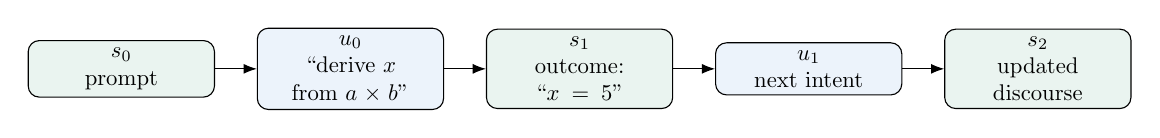
\begin{tikzpicture}[scale=0.82,transform shape,node distance=0.55cm and 0.65cm,>=Latex,
  box/.style={draw,rounded corners,align=center,minimum height=0.8cm,
              text width=2.65cm},
  act/.style={box,fill=cblue!9}, state/.style={box,fill=cgreen!9}]
\node[state] (s0) {$s_0$\\prompt};
\node[act,right=of s0] (a0) {$u_0$\\``derive $x$ from $a\times b$''};
\node[state,right=of a0] (s1) {$s_1$\\outcome: ``$x=5$''};
\node[act,right=of s1] (a1) {$u_1$\\next intent};
\node[state,right=of a1] (s2) {$s_2$\\updated discourse};
\draw[->] (s0)--(a0); \draw[->] (a0)--(s1);
\draw[->] (s1)--(a1); \draw[->] (a1)--(s2);
\end{tikzpicture}
\end{center}

The intent sentence contains operands and the operation, but not the answer.
Consequently, predicting $s_{t+1}$ requires modelling the consequence rather
than copying outcome tokens.

\medskip
A \textbf{distractor} is a feasible computation unrelated to the queried
quantity. It may be locally valid while wasting planning budget.
\end{frame}

\begin{frame}{Evaluation protocol}
\small
\begin{tabular}{p{0.24\textwidth}p{0.69\textwidth}}
\toprule
Candidate interface & Every policy scores all currently feasible intent
sentences. This interface is identical for JEPA and language-model baselines.\\
Closed-loop planning & Execute one action, observe the true rendered outcome,
re-encode the state, and replan.\\
Optimal action budget & Exactly $n$ executions for a problem with $n$ necessary
computations. Any distractor is fatal.\\
+2-action budget & At most $n+2$ executions. A successful trace can contain no
more than two distractors.\\
Selection protocol & Choose objectives on validation data; evaluate the
frozen model once on a disjoint generated test split.\\
Reporting & Three independent seeds for the final model, each final
one-component ablation, and every principal baseline.\\
\bottomrule
\end{tabular}
\end{frame}

\begin{frame}{Matched policy baselines}
\small
\begin{tabular}{p{0.37\textwidth}p{0.56\textwidth}}
\toprule
Method & Decision rule\\
\midrule
Random feasible policy & Uniform choice from the shared candidate set.\\
Autoregressive token policy & Mean token log-likelihood of each intent phrase,
conditioned on the prompt and executed history.\\
Autoregressive sentence policy & Mean token cross-entropy of each intent.\\
Sentence policy + latent prediction & Intent likelihood with an auxiliary
next-sentence latent target.\\
Latent dynamics model & Predict $F(s_t,u)$ and minimize its learned planning
energy.\\
Symbolic preference reference & Same latent model, but action pairs are
ordered by exact remaining computations; this is an annotated reference, not
the proposed non-symbolic method.\\
\bottomrule
\end{tabular}

\medskip
Historical LMs that score fully rendered candidate outcomes are retained only
as privileged diagnostics because those strings expose computed values.

\medskip
Completed three-seed validation: token policy
$0.827\pm0.003/0.978\pm0.003$; sentence likelihood
$0.690\pm0.053/0.903\pm0.039$; adding latent prediction gives
$0.817\pm0.034/0.953\pm0.010$ by likelihood and
$\mathbf{0.840\pm0.017}/0.965\pm0.013$ by latent distance. The annotated
reference reaches $0.962\pm0.013/0.997\pm0.003$. The reduced non-symbolic
model reaches $0.797\pm0.008/0.963\pm0.008$ over three seeds. These are
one-step, information-matched validation results; the final test remains
sealed while the flat paper matrix is completed.
\end{frame}

\begin{frame}{Intent-conditioned latent dynamics}
\begin{center}
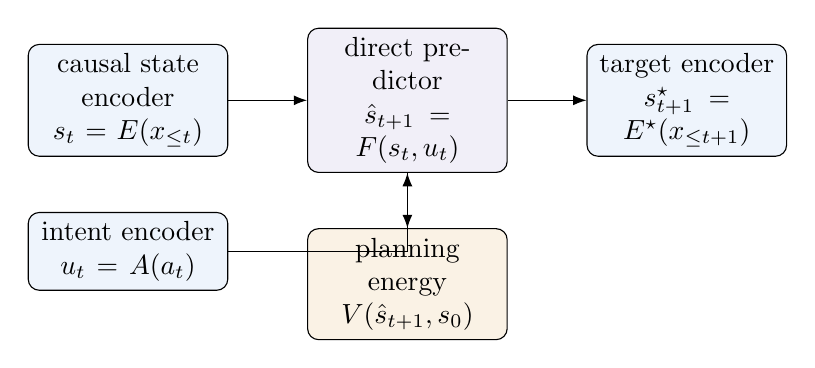
\begin{tikzpicture}[>=Latex,node distance=0.7cm and 0.8cm,
  box/.style={draw,rounded corners,align=center,minimum height=0.9cm,
              text width=2.3cm},
  enc/.style={box,fill=cblue!8}, pred/.style={box,fill=cviolet!8},
  loss/.style={box,fill=corange!10}]
\node[enc] (state) {causal state encoder\\$s_t=E(x_{\leq t})$};
\node[enc,below=of state] (action) {intent encoder\\$u_t=A(a_t)$};
\node[pred,right=1.0cm of state] (f) {direct predictor\\$\hat s_{t+1}=F(s_t,u_t)$};
\node[enc,right=1.0cm of f] (target) {target encoder\\$s_{t+1}^{\star}=E^\star(x_{\leq t+1})$};
\node[loss,below=of f] (energy) {planning energy\\$V(\hat s_{t+1},s_0)$};
\draw[->] (state)--(f); \draw[->] (action)-|(f);
\draw[->] (f)--(target);
\draw[->] (f)--(energy);
\end{tikzpicture}
\end{center}

In the over-complete model, replacing the residual parameterization by direct
next-state prediction raises optimal-budget validation accuracy from .750 to
.800. This result is not transported across objective sets: residual versus
direct prediction must be reported as a matched ablation around whichever
final objective set is selected.
\end{frame}

\begin{frame}{Supervision taxonomy}
\small
\begin{tabular}{p{0.23\textwidth}p{0.32\textwidth}p{0.36\textwidth}}
\toprule
Tier & Available information & Examples\\
\midrule
Trace-only & Observed text and learned geometry & latent prediction,
observed-action displacement decoding, terminal-distance comparisons\\
Environment interaction & Feasible actions and their rendered outcomes, but
no quality annotation & counterfactual transition augmentation; geometric
continuation teacher\\
Symbolic annotation & Task-specific relevance, remaining-step counts, or
operation classes & exact preference ranking; scalar value regression;
historical hybrid displacement labels\\
\bottomrule
\end{tabular}

\medskip
The selected objective set may use the first two tiers. Symbolic supervision is shown
only as a reference and ablation boundary.
\end{frame}

\begin{frame}{Multi-step latent-goal preference distillation}
\small
At one training state, compare the demonstrated root action with $K$ sampled
feasible alternatives. For each root $u_i$, construct an $H$-transition
continuation using only environment interaction and target geometry:
\[
q_{H,B}(u_i)=\min_{\pi\in\mathcal B_B(u_i)}
d\!\left(E^\star(x_{\leq t+H}^{\pi}),E^\star(g_{\rm trace})\right).
\]
At every continuation state, execute and target-encode every feasible child;
$\mathcal B_B$ retains the $B$ closest histories independently for each root.
Train the planning energy to preserve the resulting pairwise order.

\medskip
\begin{itemize}
\item $H$ counts transitions including the root; $B=1$ is greedy continuation.
\item $K$ counts alternatives, so training compares $K+1$ root actions.
\item The teacher never reads remaining-step counts or relevance labels.
\item The goal is a demonstrated terminal state, so distractor-contaminated
traces can make the proxy trajectory-specific.
\end{itemize}
\end{frame}

\begin{frame}{Observed-action displacement decoding}
\small
The decoder reconstructs the complete observed action phrase from the latent
displacement alone:
\[
\hat a_t=D(s_{t+1}-s_t),\qquad
\mathcal L_{\rm LDAD}=\operatorname{CE}(\hat a_t,a_t).
\]
It receives neither endpoint, the action embedding, nor an operation label.
The head is removed at inference.

\medskip
The long-horizon extension reconstructs an ordered action sequence:
\[
D_H(s_{t+H}-s_t)\rightarrow(a_t,\ldots,a_{t+H-1}).
\]
This is the discrete-text analogue of raw-action LDAD; it is kept conceptually
separate from inferred latent-action objectives.
\end{frame}

\begin{frame}{Fixed-point objective selection}
\small
Start from a deliberately over-complete non-symbolic candidate and repeat:
\begin{enumerate}
\item Remove each remaining component individually.
\item Measure optimal-budget and +2-action validation accuracy.
\item Remove components whose worst loss is at most 0.02.
\item For effects in $(0.02,0.05]$, compare a matched second-seed reference
and ablation.
\item After replication, retain the component if its mean worst-case loss
exceeds 0.02; otherwise remove it.
\item Combine accepted removals and begin another round around the smaller
model.
\end{enumerate}

Stop only when every remaining component has a reproducible measurable effect.
No auxiliary---including terminal monotonicity, hierarchy, EMA, or
open-loop prediction---has protected status.
\end{frame}

\begin{frame}{First-round component elimination}
\small
\centering
\begin{tabular}{lrrr}
\toprule
Candidate modification & optimal & +2 actions & value $\tau$\\
\midrule
over-complete objective set & 0.750 & 0.940 & 0.847\\
remove raw-action displacement decoding & 0.755 & \good{0.960} & 0.874\\
remove open-loop latent prediction & \good{0.840} & \good{0.970} & 0.920\\
remove geometry-to-value regression$^{\dagger}$ & 0.800 & 0.920 & 0.884\\
remove terminal monotonicity & 0.780 & 0.950 & 0.894\\
remove on-trajectory outcome prediction & \bad{0.680} & 0.940 & 0.800\\
remove variance--covariance regularization & \bad{0.455} & \bad{0.765} & 0.680\\
remove residual transition skip & 0.800 & \good{0.960} & 0.891\\
remove EMA target network & \bad{0.575} & \bad{0.840} & 0.735\\
remove macro-transition prediction & 0.765 & 0.940 & 0.874\\
remove counterfactual transition prediction & 0.755 & 0.935 & 0.858\\
\bottomrule
\end{tabular}

\medskip
\warn{Validation screen; table is seed 1.} Seven removals were provisionally
selected; outcome prediction, variance--covariance regularization, and EMA
were retained. $^{\dagger}$At
seed 2, removing geometry regression changes .785$\rightarrow$.680 optimal-budget;
removing faithful displacement decoding changes .785$\rightarrow$.720.
Matched reduced-model add-backs reject both terms: the reduced objective set is
better without scalar geometry regression or raw-action reconstruction.
Combining the provisional removals improves the reference from 0.750/0.940 to
\good{0.805/0.970}. A second removal round retains each remaining term.
\end{frame}

\begin{frame}{Remaining objectives have distinct functions}
\footnotesize
\centering
\begin{tabular}{lrrrr}
\toprule
Intervention & optimal & +2 actions & transition match & value $\tau$\\
\midrule
none & \good{.805} & \good{.970} & \good{.997} & \good{.904}\\
latent-state prediction & \bad{.495} & \bad{.825} & \bad{.265} & .671\\
latent-goal preference & \bad{.115} & \bad{.500} & .979 & \bad{.080}\\
outcome prediction$^{\dagger}$ & .750 & .942 & 1.000 & .856\\
predicted-outcome rollout$^{\dagger}$ & .772 & .933 & .998 & .873\\
variance--covariance regularization & \bad{.615} & \bad{.755} & .953 & .790\\
EMA target network & \bad{.720} & \bad{.910} & .987 & .871\\
add geometry-to-value regression$^{\dagger}$ & .750 & .960 & .999 & .844\\
add raw-action reconstruction$^{\dagger}$ & .788 & .958 & .999 & .871\\
\bottomrule
\end{tabular}

\medskip
\raggedright
Latent-state prediction identifies action-conditioned transitions; the
preference objective converts those transitions into a policy. Outcome
targets leave transition identity intact but sharpen the selection energy and
improve accuracy after an earlier distractor. Variance--covariance
regularization remains load-bearing in the reduced model, affecting both
transition organization and selection. EMA is also retained: its removal
degrades both budgets and off-history recovery. Adding scalar geometry
regression loses .048 optimal-budget accuracy over two seeds and remains absent. Faithful
raw-action reconstruction also remains absent: its two-seed mean is
.788/.958 versus .798/.968 without it. Both outcome
terms are retained by matched two-seed comparisons. Removing the
full target loses 0.048/0.025 under the optimal/+2 budgets; removing only its internal
predicted-outcome rollout loses 0.025/0.035. $^{\dagger}$Two-seed means; the
remaining rows are seed 1.
\end{frame}

\begin{frame}{Terminal-distance monotonicity fails under distractors}
\small
The constraint asks every demonstrated transition to approach the particular
trace-terminal embedding. A distractor may satisfy this geometric statement
because that terminal state also contains the distractor outcome, while making
no progress toward the query.

\medskip
\centering
\begin{tabular}{lrr}
\toprule
$H=4$ teacher stratum & oracle top-1 & pairwise $\tau_a$\\
\midrule
demonstrations without distractors & \good{1.000} & \good{0.898}\\
demonstrations with distractors & \bad{0.722} & \bad{0.228}\\
\bottomrule
\end{tabular}

\medskip
Removing the constraint currently outperforms retaining it with zero margin
(0.780/0.950 versus 0.765/0.940). It is therefore excluded from the combined
model and every subsequent removal round.
\end{frame}

\begin{frame}{Longer greedy continuation is not automatically better}
\small
\centering
\begin{tabular}{lrrrr}
\toprule
Teacher horizon & continuation after root & teacher top-1 & optimal & value $\tau$\\
\midrule
$H=1$ & 0 & 0.750 & \bad{0.315} & 0.542\\
$H=2$ & 1 & \good{0.930} & \good{0.750} & \good{0.847}\\
$H=4$ & 3 & 0.900 & 0.695 & 0.792\\
$H=8$ & 7 & 0.830 & 0.620 & 0.728\\
$H=16$ & 15 & 0.790 & 0.655 & 0.768\\
\bottomrule
\end{tabular}

\medskip
\raggedright
$H=1$ shows that at least one environment continuation is necessary; this
horizon is independent of hierarchy and open-loop prediction. Beyond $H=2$,
all width-one teachers remain worse. Potential causes are distinct:
\begin{itemize}
\item trajectory-specific terminal embeddings;
\item error accumulation in geometry-greedy continuation;
\item emitted preferences between actions tied under the task metric;
\end{itemize}

\scriptsize Holding the current reduced checkpoint fixed confirms $H=2$ as
the width-one optimum. Bounded continuation search changes the diagnosis:
at $H=4$, beam width 1/4/8 raises teacher top-1 .810/.870/.900 and pairwise
$\tau_a$ .646/.701/.728; the paired $H=2,B=1$ reference is .865/.661.
At $H=8/16,B=8$, top-1 is .900/.895 and $\tau_a$ is .670/.672, so extending
beyond four steps does not improve the teacher. Beam search remains
non-symbolic and costs $O((K+1)HBA)$ target encodings, where $A$ is mean
feasible branching. The matched $H=2$ root sweep selects $K=2$ alternatives;
longer teachers are not promoted by this audit.
\end{frame}

\begin{frame}{Margin tuning does not improve action selection}
\small
\centering
\begin{tabular}{lrrrr}
\toprule
Intervention & optimal & +2 actions & oracle-order top-1 & value $\tau$\\
\midrule
margin 0.5 (2-seed mean) & \good{.798} & \good{.968} & \good{.946} & \good{.894}\\
margin 0.25 (2-seed mean) & .763 & \good{.968} & .941 & .864\\
preference margin 1.0 & \bad{.575} & .870 & .888 & .781\\
preference margin 2.0 & \bad{.435} & .875 & .820 & .625\\
geometry filter .005 & .740 & .925 & .943 & .874\\
distractor mixture .30 & .790 & .935 & .940 & .882\\
scalar geometry regression$^{\dagger}$ & .750 & .960 & .928 & .844\\
\bottomrule
\end{tabular}

\medskip
\raggedright
The apparent seed-1 +2-action gain from margin .25 does not replicate: its
two-seed optimal-budget mean is .035 lower with no +2-action gain. Margins 1/2 widen the
median energy gap to .920/1.477 while reducing clean-history top-1 to
.844/.749: they make the wrong order more confident. Retain margin .5.
$^{\dagger}$Two-seed mean.
\end{frame}

\begin{frame}{LDAD separates collapse prevention from transition identity}
\scriptsize
\centering
\begin{tabular}{llrrrr}
\toprule
Target & regularizer & state std (off/on) & rank (off/on) & match (off/on) & RSA (off/on)\\
\midrule
EMA & none & .457/.294 & 83.0/97.6 & .432/\good{.959} & .300/.737\\
online + stop-grad & none & .102/.343 & 2.9/101.8 & .299/\good{.963} & .406/.785\\
fully online & none & .000/.145 & 97.1/90.3 & .322/\good{.988} & .529/.778\\
fully online & VICReg & 1.016/1.007 & 234.5/219.6 & .334/\good{.980} & .558/.909\\
fully online & SIGReg & .980/.975 & 94.2/103.9 & .951/.998 & .972/.956\\
\bottomrule
\end{tabular}

\medskip
VICReg can produce healthy scale and rank without identifying
action-conditioned transitions. LDAD supplies transition identity; it does
not by itself guarantee a calibrated planning energy. In the matched official
symbolic-preference pilot, LDAD off/on raises transition matching
.889$\rightarrow$.956 but changes optimal-budget success .565$\rightarrow$.535 and
clean/after-error top-1 .848/.653$\rightarrow$.837/.623.
\end{frame}

\begin{frame}{Minimal two-objective text Delta-JEPA control}
\small
All rows use fully online gradients and unnormalized latent MSE, without EMA,
stop-gradient, VICReg, SIGReg, outcome anchoring, hierarchy, or planning
supervision.

\medskip
\centering
\begin{tabular}{lrrrr}
\toprule
Action objective & state std & state rank & transition match & RSA\\
\midrule
none & \bad{0.00028} & 95.8 & \bad{0.307} & 0.466\\
adjacent raw-action LDAD & \good{0.117} & 89.5 & \good{0.975} & 0.775\\
four-action sequence LDAD & \good{0.080} & 140.1 & \good{0.994} & 0.804\\
\bottomrule
\end{tabular}

\medskip
Raw-action displacement decoding prevents magnitude collapse and makes
counterfactual transitions identifiable in the intended minimal setting.
\end{frame}

\begin{frame}{Residual errors arise from action ordering}
\scriptsize
Both models identify counterfactual next states nearly perfectly. Symbolic
preferences primarily improve their energy ordering, not transition identity.

\medskip
\centering
\begin{tabular}{lrrrr}
\toprule
Preference target & transition match & value $\tau$ & oracle-trace top-1 & optimal success\\
\midrule
latent-goal continuation & .997 & .904 & .948 & .805\\
latent-goal continuation, gap .005 & .997 & .874 & .943 & .740\\
symbolic action order & 1.000 & .980 & .995 & \good{.960}\\
\bottomrule
\end{tabular}

\medskip
\begin{tabular}{lrrr}
\toprule
Preference target & clean-history top-1 & after-error top-1 & median margin\\
\midrule
latent-goal continuation & .940 & .706 & .610\\
latent-goal continuation, gap .005 & .914 & .681 & .520\\
symbolic action order & \good{.989} & \good{.857} & \good{1.617}\\
\bottomrule
\end{tabular}

\medskip
\raggedright
The mean problem requires 4.07 decisions and
$0.948^{4.07}=0.804$, matching the observed 0.805. Errors are rarely ties:
only 1.2\% of competitive decisions have an absolute margin below 0.02.
Lowering the geometric tie filter to .005 degrades ordering and success, so
the added small-distance comparisons are noisy rather than useful coverage.
The remaining gap is a calibrated action-selection problem, with additional
amplification after the first off-trajectory action.
\end{frame}

\begin{frame}{Faithful iGSM transfer: separate model selection}
\small
The faithful domain uses the official generator and renderer rather than the
stylized mod-23 environment. It changes sentence length, operation structure,
graph depth, and action identifiers.

\medskip
The transfer protocol repeats the complete scientific procedure:
\begin{enumerate}
\item initialize from the selected stylized model;
\item screen exact component additions: require a gain above .02, reject any
budget loss above .02, and replicate gains in .02--.05;
\item repeat iterative one-component elimination to a fixed point;
\item compare matched autoregressive, random, symbolic-reference, and latent
world-model policies over three seeds;
\item evaluate the frozen model on a disjoint official-iGSM test set.
\end{enumerate}
\end{frame}

\begin{frame}{Faithful iGSM: sentence likelihood is the strongest current baseline}
\small
\centering
\begin{tabular}{lrr}
\toprule
One-seed validation policy & optimal & +2 actions\\
\midrule
random feasible selection & .200 & .460\\
token intent likelihood & .415 & .675\\
sentence intent likelihood & .450 & .755\\
sentence likelihood + latent prediction & \good{.455} & \good{.765}\\
same model, latent-distance selection & .445 & .715\\
symbolic-preference latent reference & .565 & .805\\
\bottomrule
\end{tabular}

\medskip
\raggedright
The auxiliary next-latent target changes likelihood selection by only
.005/.010, and its latent distance is a worse selection score. Unlike the
stylized domain, token-level likelihood also trails sentence likelihood.
No official-iGSM configuration is frozen from these baseline rows; hierarchy
is being resolved first in the faster stylized environment.
\end{frame}

\begin{frame}{Variational studies are a separate question}
\small
\begin{tabular}{p{0.23\textwidth}p{0.22\textwidth}p{0.20\textwidth}p{0.18\textwidth}}
\toprule
Model & Action at training & Next-state target & Scientific question\\
\midrule
deterministic discourse JEPA & observed intent sentence & deterministic latent & selected planning model\\
probabilistic discourse JEPA & observed intent sentence & diagonal Gaussian & uncertainty with known actions\\
action-free sentence stream & inferred posterior code & diagonal Gaussian & can transition modes emerge without actions?\\
\bottomrule
\end{tabular}

\medskip
In the action-free model, $q(u_t\mid s_t,s_{t+1})$ observes the outcome. A
learned prior $p(u_t\mid s_t)$ must recover a usable code before the outcome
exists. Decoding the posterior code from $s_{t+1}-s_t$ is therefore not
raw-action LDAD.
\end{frame}

\begin{frame}{Observed-action variational LDAD does not prevent collapse}
\small
All cells below use a probabilistic next-state target, no VICReg/SIGReg, and
the same observed intent action. Values show raw LDAD off/on.

\medskip
\centering
\begin{tabular}{lrrrr}
\toprule
Target gradient path & state std & shuffle ratio & LDAD-on token/exact & residual$^2$\\
\midrule
online stop-gradient & .00075 / .00454 & 1.004 / 1.152 & .898 / .582 & 1.006 / 1.012\\
fully online & .00034 / .00305 & 1.000 / 1.035 & .900 / .583 & 1.004 / 1.007\\
\bottomrule
\end{tabular}

\medskip
\scriptsize VICReg here means variance--covariance stabilization; SIGReg is a
random-projection Gaussianity regularizer.\par
\smallskip
\raggedright
The decoder recovers the observed sentence by amplifying tiny displacement
directions, while learned variance calibrates a collapsed target mean.
Consequently, faithful LDAD alone does not transfer the deterministic
anti-collapse result to probabilistic states; EMA and explicit distributional
regularization must be tested separately.
\end{frame}

\begin{frame}{EMA and SIGReg expose action-conditioned uncertainty}
\small
All rows use probabilistic next-state prediction and pooled observed intents.
Values show raw-action LDAD off/on.

\medskip
\centering
\begin{tabular}{lrrrr}
\toprule
Target / regularizer & state std & state rank & matched L1 & shuffle ratio\\
\midrule
EMA / none & .062/.286 & 76.4/52.3 & .003/.008 & 1.182/1.455\\
EMA / VICReg & .844/.906 & 97.2/90.1 & .016/.018 & 1.226/1.647\\
EMA / SIGReg & .977/.970 & 104.5/80.2 & .418/\good{.062} & 1.375/\good{2.293}\\
official EMA / SIGReg & .981/.979 & 119.7/102.9 & .463/\good{.067} & 1.105/\good{1.462}\\
online stop-gradient / SIGReg & .973/.946 & 88.5/45.1 & .424/.008 & 1.398/1.219\\
\bottomrule
\end{tabular}

\medskip
EMA+SIGReg+LDAD gives healthy state scale and stronger observed-action
dependence on both stylized and independently rendered official text. LDAD
does not universally raise rank; action sensitivity, predictive error, and
state geometry must all be reported.
\end{frame}

\begin{frame}{A scalar schedule recalibrates long-horizon spread}
\scriptsize
The true intent sequence is fixed; 32 Gaussian trajectories are propagated
recursively. One standard-deviation multiplier per horizon is fitted on 500
validation trajectories, then frozen and applied to 1,000 disjoint test
trajectories.

\medskip
\centering
\begin{tabular}{llrrrrr}
\toprule
Domain & LDAD & $H$ & open-loop L1 & raw 2$\sigma$ & multiplier & calibrated 2$\sigma$\\
\midrule
stylized & off & 4 & .533 & .990 & .742 & \good{.953}\\
stylized & on  & 4 & \good{.144} & \bad{.882} & 1.308 & \good{.954}\\
official & off & 8 & .655 & .998 & .612 & \good{.953}\\
official & on  & 8 & \good{.276} & \bad{.776} & 1.684 & \good{.952}\\
\bottomrule
\end{tabular}

\medskip
\raggedright
Raw-action reconstruction sharply improves conditional transition means. Its
long-horizon under-dispersion is largely a scalar scale error: across all
reported test cells, calibrated residual squared is .964--1.084 and two-sigma
coverage is .943--.962. The scalar does not correct accumulated mean bias, so
transition fidelity and uncertainty calibration remain distinct.
\end{frame}

\begin{frame}{Same-state audit: broad support is not accurate control}
\scriptsize
For each state, encode every feasible rendered outcome. ``Distinct'' means a
prediction enters the ball whose radius is half the distance to the nearest
competing outcome; ``precise'' additionally requires posterior-level error.

\medskip
\centering
\begin{tabular}{llrrrr}
\toprule
Domain / target & posterior-code rec. & outcome sep. & posterior distinct & prior distinct & prior precise\\
\midrule
stylized / stop-grad.+SIGReg & off & .706 & .285 & .052 & .004\\
stylized / stop-grad.+SIGReg & on & .665 & \good{.645} & \good{.278} & .016\\
stylized / zero free nats & off & .774 & \bad{.006} & \bad{.010} & .010\\
stylized / four-component prior & off & .703 & .230 & .050 & .005\\
official / EMA+VICReg & off & .005 & .000 & .000 & .000\\
official / stop-grad.+SIGReg & off & \good{.989} & \good{.753} & \good{.598} & .073\\
official / stop-grad.+SIGReg & on & .743 & \good{.838} & \good{.675} & .029\\
\bottomrule
\end{tabular}

\medskip
\raggedright
Posterior-code reconstruction separates outcome-informed modes and broadens
support, but does not make it precise: on official iGSM it reduces precise
coverage from .073 to .029 while improving broad coverage from .598 to .675.
EMA+VICReg appears healthy globally while collapsing same-state alternatives;
stop-gradient+SIGReg preserves alternatives but lacks a goal-directed prior.
Forcing posterior--prior alignment by removing free nats collapses the learned
action modes, so stronger KL is not pursued. A four-component Gaussian prior
also collapses to 1.36 effective components and does not improve coverage;
additional prior capacity cannot identify unseen same-state alternatives.
\end{frame}

\begin{frame}{Architecture changes the probabilistic trade-off}
\scriptsize
All rows use EMA and the same 16-dimensional observed-action code. The ordered
representation retains two dimensions per token; the direct predictor removes
the residual state skip.

\medskip
\centering
\begin{tabular}{lllrrrr}
\toprule
Reg. & action representation & predictor & LDAD & matched L1 & shuffle ratio & state rank\\
\midrule
SIG & pooled & residual & on & \good{.062} & 2.293 & 80.2\\
SIG & ordered tokens & residual & on & .102 & 2.086 & 89.3\\
SIG & pooled & direct & off & .501 & 1.728 & 161.4\\
SIG & pooled & direct & on & .245 & \good{2.990} & 171.8\\
VIC & pooled & residual & on & \good{.018} & 1.647 & 90.1\\
VIC & pooled & direct & off & .469 & 1.415 & \good{221.1}\\
VIC & pooled & direct & on & .320 & 1.835 & \good{213.6}\\
\bottomrule
\end{tabular}

\medskip
Ordered-token concatenation does not improve the selected setting. Direct
prediction retains richer state geometry under both regularizers; residual
prediction achieves the lowest error. SIGReg favors action dependence, while
VICReg favors effective state rank. On official iGSM, direct-predictor LDAD
reproduces the effect: matched L1 .719$\rightarrow$.266 and shuffle ratio
1.097$\rightarrow$1.457 at state rank 163.5. The ordered-token transfer is
also negative: relative to pooled LDAD, exact phrase recovery improves
.730$\rightarrow$.775, but action-code rank halves 14.5$\rightarrow$7.8,
matched L1 worsens .067$\rightarrow$.081, and the shuffle ratio falls
1.462$\rightarrow$1.222. Official VICReg direct prediction confirms the
trade-off: LDAD changes error .612$\rightarrow$.199 and sensitivity
1.104$\rightarrow$1.307 while retaining state rank 197.3. SIGReg yields
stronger action dependence; VICReg yields lower error and richer geometry.
\end{frame}

\begin{frame}{Direct prediction does not replace the target network}
\small
Fully online gradients with SIGReg; values show raw-action reconstruction
off/on. A healthy representation requires scale, rank, and conditional action
dependence simultaneously.

\medskip
\centering
\begin{tabular}{lrrrr}
\toprule
Predictor & state rank & action rank & matched L1 & shuffle ratio\\
\midrule
residual & 14.1/17.5 & 11.6/11.5 & .001/.002 & 1.054/1.138\\
direct & \bad{8.5/6.3} & \bad{1.27/1.42} & .004/.005 & 51.4/48.3\\
\bottomrule
\end{tabular}

\medskip
The large direct-predictor ratios are denominator effects: matched error is
almost zero while action dependence occupies approximately one direction.
Neither the direct architecture nor displacement-to-action reconstruction
prevents low-rank collapse without a stabilized target network.
\end{frame}

\begin{frame}{Hierarchical control protocol}
\small
Three observed intent actions are compressed into one macro action,
and the high-level dynamics predict the corresponding state transition:
\[
m_t=q_\phi(a_{t:t+2}),\qquad
\hat z_{t+3}=F_{\rm hi}(z_t,m_t).
\]

$F_{\rm hi}$ is a two-layer causal transformer that retains the complete
macro-state/action history during autoregressive rollout. The primitive
$F_{\rm low}$ is a Markov state--action MLP applied recursively; it does not
attend to an explicit sequence of earlier primitive states.

\begin{enumerate}\itemsep2pt
\item \textbf{High-level planning.} CEM optimizes a sequence of macro actions,
propagates them through $F_{\rm hi}$, and scores the predicted macro states.
Reported runs use 1,200 candidates, 20 refits, 10 elites, and variance EMA
0.9---within the hundreds-to-thousands/5--40-iteration HWM regime.
\item \textbf{Support control.} A conditional macro prior and a separately
learned support score penalize implausible actions. Encoded terminal-state
distance uses the solved trace as an oracle goal observation: it reproduces
the HWM objective, but is not deployable when the answer is unknown. Exact
graph distance is also labeled as oracle supervision wherever it trains a value.
\item \textbf{Closed-loop refinement.} The first predicted macro state becomes
a subgoal for $Q_{\rm low}(z,a,z_{\rm subgoal})$, which scores only actions
feasible \emph{now}. One primitive action is executed and both levels replan.
Near termination, a learned remaining-cost threshold switches to flat control.
\end{enumerate}

No future feasible-action sequence is supplied to the deployed planner.
\end{frame}

\begin{frame}{Dense supervision improves recursive dynamics}
\small
The recursive shifted-sequence loss supervises every valid origin at every
horizon, rather than only a rollout from the initial state.

\medskip
\begin{columns}[T,onlytextwidth]
\column{0.48\textwidth}
\centering
\textbf{High-level LN--L1 error}\par
\begin{tabular}{lrrr}
\toprule
supervised depth $N$ & $h=1$ & $h=2$ & $h=3$\\
\midrule
none & .586 & .629 & .684\\
1 & \good{.557} & .600 & .660\\
2 & .559 & .580 & .631\\
3 & .560 & \good{.578} & \good{.622}\\
\bottomrule
\end{tabular}

\column{0.48\textwidth}
\centering
\textbf{Low-level LN--L1 error}\par
\begin{tabular}{lrrr}
\toprule
supervised depth $N$ & $h=1$ & $h=4$ & $h=8$\\
\midrule
none & .493 & .637 & .867\\
1 & \good{.470} & .590 & .707\\
4 & .477 & \good{.552} & .614\\
8 & .480 & .553 & \good{.604}\\
\bottomrule
\end{tabular}
\end{columns}

\medskip
On the same 200 long-tail problems, flat success changes from .300 to
.335/.355/.345 for $N=1/4/8$. Thus $N=4$ is the behavioral choice even though
$N=8$ has the lowest eight-step prediction error. Better prediction is
necessary but is not itself evidence that hierarchical control works.
\end{frame}

\begin{frame}{State-value distillation is better calibrated than latent distance}
\footnotesize
All rows rank 11,659 valid macro spans at 200 held-out states. Exact remaining
computations supervise the learned-value rows, so this is an
\emph{oracle-supervised diagnostic}, not the non-symbolic headline model.

\medskip
\centering
\begin{tabular}{lrrrr}
\toprule
High-level score & correlation & pair accuracy & top-1 optimal & regret\\
\midrule
terminal latent distance (oracle goal observation) & .478 & .591 & .590 & .545\\
macro action value $Q(z,m)$ & .727 & .694 & .715 & .405\\
state value $V(z')$, factual regression & .857 & .729 & .790 & .295\\
$V(z')$ + counterfactual regression & \good{.860} & .734 & \good{.800} & \good{.280}\\
$V(z')$ + regression + pairwise rank & .859 & \good{.735} & \good{.800} & \good{.280}\\
\bottomrule
\end{tabular}

\medskip
The next-state value is substantially better calibrated than latent goal
distance. Counterfactual regression helps slightly; an additional ranking
hinge does not improve top-1 selection. A support classifier separates valid
from three-standard-deviation perturbations almost perfectly, yet this offline
separation does not by itself improve control.
\end{frame}

\begin{frame}{A validation depth curve is not a hierarchy result}
\footnotesize
Dense high-level supervision and the recalibrated state value produce the
first monotone planning-depth curve, but only on the 100-problem selection
screen.

\medskip
\centering
\begin{tabular}{lrrr}
\toprule
High-level score & one macro step & two macro steps & three macro steps\\
\midrule
learned state value $V(z')$ & .260 & .300 & \good{.330}\\
terminal latent distance (oracle goal observation) & .310 & .310 & .310\\
matched flat controller & .280 & .280 & .280\\
\bottomrule
\end{tabular}

\medskip
The learned value benefits from deeper recursive prediction; the HWM-style
latent terminal distance does not. This table is a model-selection diagnostic:
one dataset, one checkpoint lineage, and only 100 episodes. It motivates a
larger paired confirmation; it cannot establish a positive hierarchy effect.
\end{frame}

\begin{frame}{Continuous latent-action hierarchy does not confirm}
\small
The selected setting uses low-level dense depth 4, high-level dense depth 3,
the counterfactually trained state value, a soft support penalty, and
three-step macro planning. Each row evaluates the flat and hierarchical
controllers on the same 500 newly generated 7--9-step problems.

\medskip
\centering
\begin{tabular}{lrrrr}
\toprule
data / planner seed & flat & hierarchy & difference & macro decisions\\
\midrule
31 / 731 & .314 & .272 & -.042 & .633\\
32 / 732 & .336 & .320 & -.016 & .623\\
33 / 733 & .322 & .274 & -.048 & .634\\
\midrule
mean & \good{.324} & \bad{.289} & \bad{-.035} & .630\\
\bottomrule
\end{tabular}

\medskip
The 100-problem .33 versus .28 comparison was selection noise. Continuous
latent-vector optimization followed by low-level subgoal refinement is 3.5
points worse on average and increases distractor selection. This rejects that
particular HWM-style interface; it does not reject hierarchy in general.
\end{frame}

\begin{frame}{What the hierarchy diagnostics rule out}
\footnotesize
\begin{tabular}{p{0.24\textwidth}p{0.44\textwidth}p{0.24\textwidth}}
\toprule
Hypothesis & Decisive observation & Status\\
\midrule
CEM is under-budgeted & 1,200 candidates $\times$ 20 refits strongly reduces
its objective; larger-scale HWM settings are already used. & not supported\\
Arbitrary macro vectors are the sole failure & action banks, nearest-code
projection, conditional-prior noise, local GMMs, support penalties, and
epistemic disagreement do not improve confirmed success. & not primary\\
Recursive dynamics are too weak & dense supervision reduces high $h=3$ error
.684$\to$.622 and low $h=8$ error .867$\to$.604. & real, but insufficient\\
The high-level score is uncalibrated & exact state-value distillation raises
top-1 macro selection .590$\to$.800 relative to latent distance. & improved,
not solved\\
The lower controller cannot realize waypoints & measured endpoint residuals
and open-loop reachability costs are negative; even true-waypoint control only
matches the flat controller in the latest long-tail audit. & remaining gate\\
\bottomrule
\end{tabular}

\medskip
These findings motivate two separable tests: learn controller-specific
executability from realized lower-controller outcomes, and restrict planning
to macro actions obtained by encoding actual text spans. The former tests the
high--low interface; the latter changes the optimization domain.
\end{frame}

\begin{frame}{Controller-outcome reranking exposes the missing signal}
\footnotesize
For each continuous CEM decision, we execute the top 32 proposed subgoals for
three closed-loop low-level steps and rerank by the measured endpoint.

\medskip
\centering
\begin{tabular}{lrr}
\toprule
Reranking signal & success & interpretation\\
\midrule
matched flat / ordinary CEM & .260 / .260 & reference\\
endpoint reachability residual & .260 & geometric realizability is insufficient\\
endpoint latent-goal distance, weight 1 / 10 & .280 / .300 & modest task alignment\\
exact realized remaining work & \good{.440} & strong candidate-set headroom\\
\midrule
learned regression / pairwise / listwise score & .260 / .260 / .290 & does not recover oracle gain\\
\bottomrule
\end{tabular}

\medskip
The exact reranker changes 46\% of decisions, reduces remaining work from
3.46 to 2.90, and reduces selected distractors from .754 to .192. The failure
is therefore not lack of useful candidates: learned continuous scoring does
not identify task-progressing, controller-realizable candidates reliably.
\end{frame}

\begin{frame}{Support-constrained discrete macro planning}
\small
We next plan over encoded sequences of observed intent phrases rather than
arbitrary latent vectors:
\[
u=q_\phi(a_t,\ldots,a_{t+h-1}),\qquad
\hat z_{t+h}=F_{\rm hi}(z_t,u).
\]

\begin{enumerate}\itemsep3pt
\item Candidate sequences start with an action feasible at the current state;
later elements are drawn from unresolved problem actions. The planner is
\emph{not} given their future symbolic feasibility.
\item The high-level model recursively scores the encoded macro sequence, and
a learned state-conditioned support score penalizes implausible continuations.
\item The first text action of the selected sequence is executed directly;
the sequence is discarded and the model replans from the new observation.
\end{enumerate}

This retains a text-grounded action interface and prevents continuous
optimizer exploitation by construction. Crucially, the finite proposal bank
must be balanced over its first action: that is the action executed by
receding-horizon control. A plain lexicographic cap leaks action ordering.
\end{frame}

\begin{frame}{Candidate-order control invalidates the apparent gain}
\small
The initially reported discrete planner capped an exponentially expanding
sequence list by taking its first 512 entries. This over-represented early
first actions. Three large replications reproduced the implementation, not a
model effect.

\medskip
\centering
\begin{tabular}{lrrr}
\toprule
Stylized protocol & flat & hierarchy & first-feasible control\\
\midrule
unbalanced H2, 3$\times$500 mean & .326 & .376 & not measured\\
balanced arbitrary sequences, $n=100$ & .310 & \bad{.110} & .100\\
root-balanced learned-support beam & .310 & .150 & .100\\
$+$ one-step value, weight 1 / 10 & .310 & .250 / .300 & .100\\
\bottomrule
\end{tabular}

\medskip
The corrected implementation uses equal proposal multiplicity per current
action and reproducibly randomizes future candidates. Every evaluation now
reports the ordered-action control. No positive discrete hierarchy result is
currently supported; planning-matched feasibility closes the small screen to
within one point of flat control but does not work without a one-step value.
\end{frame}

\begin{frame}{Corrected hierarchy fails on first-action credit}
\small
All rows use root-balanced candidates on the same 100-problem selection split.

\medskip
\centering
\begin{tabular}{lrr}
\toprule
Planner signal & success & sequence validity\\
\midrule
flat one-step value & .310 & n/a\\
learned-support beam & .150 & learned proposal\\
planning-matched support + one-step value & .320 & learned proposal\\
oracle-feasible sequences, terminal macro value & .170 & \good{1.000}\\
oracle-feasible + one-step value & .330 & \good{1.000}\\
prefix-aware macro $Q$ alone, scale .1/1/5 & .170/.170/.150 & learned proposal\\
prefix-aware macro $Q$ + one-step value & .330/.330/.320 & learned proposal\\
\bottomrule
\end{tabular}

\medskip
Oracle-feasible six-action plans complete 4.7 necessary computations on
average, yet terminal scoring performs poorly. The planner values eventual
progress but executes only the first action and replans, allowing useful work
to be deferred repeatedly.
\end{frame}

\begin{frame}{Corrected paired confirmation is negative}
\small
The best safeguarded configuration was frozen after the selection screen and
evaluated on three fresh 500-problem sets. Candidate banks are root-balanced,
future proposals are reproducibly randomized, and action menus are shuffled.

\medskip
\centering
\begin{tabular}{lrrr}
\toprule
Data / planner seed & flat & hierarchy & difference\\
\midrule
71 / 871 & .318 & .310 & -.008\\
72 / 872 & .332 & .326 & -.006\\
73 / 873 & .300 & .296 & -.004\\
\midrule
mean & \good{.317} & .311 & -.006\\
\bottomrule
\end{tabular}

\medskip
The direction is negative in every pair. Hierarchical prediction is useful as
an auxiliary representation experiment, but this controller is not included
in the cumulative model recipe.
\end{frame}

\begin{frame}{Prediction improves; abstraction is not established}
\small
Dense supervision lowers high-level three-step error .684$\to$.622 and
low-level eight-step error .867$\to$.604. The learned macro-state value has
correlation .860 with remaining work, and the representations are not
collapsed: state/action/macro effective ranks are approximately
239/256, 15/16, and 21/32.

\medskip
These observations establish predictive structure and task-progress content,
not emergent semantic abstraction:
\begin{itemize}
\item recent hierarchy stages freeze the primitive state encoder, so hierarchy
cannot reorganize the base representation;
\item the high level predicts the same state space three actions later rather
than a separately bottlenecked abstract state;
\item stylized iGSM computations are largely homogeneous and commuting, with
few natural option or phase boundaries.
\end{itemize}

The appropriate abstraction test compares token-, phrase-, sentence-, and
paragraph-timescale states and measures whether higher levels discard surface
features while retaining more future-relevant reasoning variables.
\end{frame}

\begin{frame}{Faithful iGSM exposed a second ordering leak}
\small
The official graph iterates parameters in a near-topological order. Returning
feasible actions in that order silently supplies a strong solution heuristic.

\medskip
\centering
\begin{tabular}{lrrr}
\toprule
Action-menu protocol, $n=100$ long & flat & hierarchy & first feasible\\
\midrule
reference parameter order & .330 & .880 & \bad{1.000}\\
problem-specific shuffled order & .330 & .310 & .330\\
\bottomrule
\end{tabular}

\medskip
The model, prompt, problems, and feasible-action sets are unchanged; only menu
order differs. Every method now receives the same stable, problem-specific
shuffled menu and every table reports the first-feasible control. Earlier
faithful planning results using reference order are excluded and must be rerun.
\end{frame}

\begin{frame}{The earlier macro-depth curve is not valid evidence}
\small
Depth is selected on a separate 100-problem validation screen using the same
checkpoint and candidate budget.

\medskip
\centering
\begin{tabular}{lrrrrr}
\toprule
Controller & flat & H1 & H2 & H3 & H4\\
\midrule
success & .310 & .180 & \good{.410} & .390 & .330\\
\bottomrule
\end{tabular}

\medskip
All four depths used the unbalanced sequence cap. Because truncation severity
changes with sequence length, the curve conflates planning depth with which
first actions survive enumeration. It is retained only as provenance and is
excluded from model selection. Depth must be rerun after the corrected,
root-balanced proposal mechanism is fixed.
\end{frame}

\begin{frame}{What the evidence currently supports}
\begin{enumerate}
\item Intent-conditioned latent prediction supports auditable
counterfactual transitions and closed-loop reasoning.
\item Action selection, not one-step transition identity, is the main source
of residual episode failures.
\item Raw-action displacement decoding prevents deterministic collapse and
strengthens variational transition grounding, but does not by itself ensure
healthy probabilistic rank.
\item Dense low- and high-level supervision improves recursive prediction;
learned next-state values are better calibrated than latent goal distance.
Continuous latent-action CEM nevertheless fails paired confirmation.
\item Restricting macro actions to encoded text spans does not improve control:
the initial positive result was caused by first-action-biased candidate
truncation, and corrected 3$\times$500 planning is .311 versus .317 flat.
\item Inferred posterior transition codes should not be presented as usable
actions until a state-conditioned prior can retrieve or generate them. Hard-text
hierarchy remains paused. Faithful iGSM also requires a shuffled action menu:
the reference parameter iteration order is itself a topological-order leak.
\end{enumerate}
\end{frame}

\begin{frame}{Limitations and completion criteria}
\footnotesize
\begin{itemize}\itemsep1pt
\item The flat stylized model and policy baselines have three validation seeds.
The corrected hierarchical planner failed paired confirmation; the final task
test remains sealed until the flat cumulative and ablation matrix is frozen.
\item The latent-goal teacher uses environment interactions and a demonstrated
terminal state. It removes symbolic quality labels, but not the action
interface.
\item Flat lookahead beyond one step requires the reference graph to propose
future feasible actions and is therefore an oracle-action diagnostic. The
deployed discrete hierarchy uses current feasible actions only for the first
choice; future candidates are unresolved text actions, not oracle-feasible
sequences.
\item Exact remaining graph distance substantially improves the high-level
state value. It is an oracle-supervised mechanism diagnostic until a
non-symbolic target reproduces the effect.
\item HWM-style terminal latent distance requires an encoded solved-state goal
observation. That observation is available in goal-conditioned control but not
in answer-unknown reasoning, so it is an oracle diagnostic here.
\item Official iGSM requires its own objective-selection and ablation cycle; stylized
choices are hypotheses, not guaranteed transfers.
\item Probabilistic action-free models currently lack a usable action prior.
They are a separate representation study and are paused during hierarchy work.
\end{itemize}

\medskip
Root-balanced planning did not exceed matched flat control on three independent
500-problem sets, so hierarchy is excluded from the easy-domain main recipe.
Any future faithful transfer must randomize action-menu order and use a newly
predeclared protocol rather than inheriting the invalid historical result.
\end{frame}

\appendix
\begin{frame}{Appendix: artifact mapping}
\scriptsize
\begin{tabular}{p{0.55\textwidth}p{0.37\textwidth}}
\toprule
Scientific condition & Artifact family\\
\midrule
multi-step latent-goal preference distillation & \texttt{disc\_gar\_greedy\_*}\\
raw-action displacement stability factorial & \texttt{dldad\_*}\\
minimal text Delta-JEPA controls & \texttt{deltajepa\_text\_*}\\
probabilistic observed-action models & \texttt{dvjepa\_*}\\
action-free sentence stream & \texttt{svjepa\_*}\\
fair intent-policy language models & \texttt{lm\_intent}, \texttt{sentlm\_*\_intent}\\
official-iGSM transfer & \texttt{real\_*}, faithful configuration suffixes\\
dense high-level recursive supervision & \texttt{intent\_hidense\_tail79\_n*}\\
dense low-level recursive supervision & \texttt{intent\_lodense\_tail79\_n*}\\
macro-state value calibration & \texttt{intent\_hivalue\_tail79\_*}\\
paired hierarchy confirmation & \texttt{confirm\_ds*\_s*\_\{flat,hier\}.json}\\
controller-outcome diagnostics & \texttt{intent\_controller\_outcomes/*}\\
discrete hierarchy confirmation & \texttt{confirm\_ds*\_s*\_\{h2,discrete\_h3\}.json}\\
\bottomrule
\end{tabular}
\end{frame}

\begin{frame}{Appendix: diagnostics reported for every final model}
\small
\begin{itemize}
\item optimal-budget and +2-action closed-loop success;
\item chosen-action distractor rate;
\item counterfactual transition nearest-neighbour matching and RSA;
\item value-energy pairwise $\tau$ and oracle-order top-1;
\item state scale and effective rank;
\item observed-action token and exact-phrase recovery when LDAD is present;
\item probabilistic NLL, standardized residual, and one/two-sigma coverage;
\item posterior/prior semantic probes and retrieval for inferred actions.
\end{itemize}
\end{frame}

\end{document}
